\chapter{相关工作}

为了更好地设计适用于日常健康场景下的面诊系统,本章将介绍当前比较流行的基于面诊技术的面诊系统以及当前人机交互领域中日常健康场景的相关研究。

\section{面诊系统}

面诊系统是基于面诊算法为用户提供面诊功能的一套系统。
目前已经有不少研究将面诊技术落地,大致可以分为以强依赖硬件设备的面诊仪和各类面诊系统,下面将主要介绍代表性的几类,同时简单概括其特点以及不足之处。

\begin{figure}[h]
    \centering
    \subfigure[面诊仪]{
        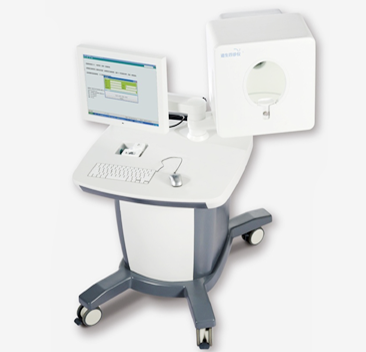
\includegraphics[width=5cm]{images/mzy.png}
    }
    \subfigure[舌面诊一体化设备]{
        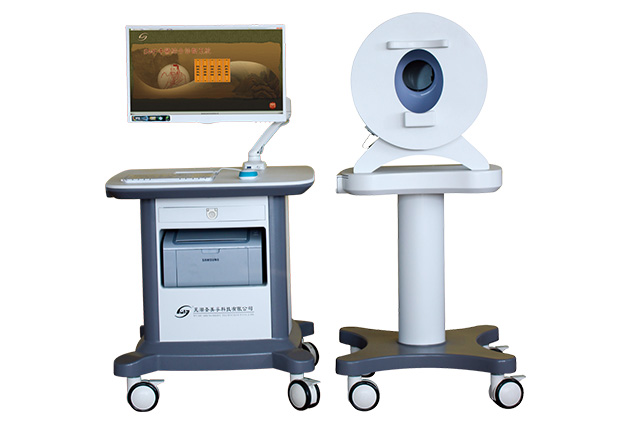
\includegraphics[width=5cm]{images/SMF.jpg}
    }
    \caption{面诊仪}
    \label{fig:med}
\end{figure}

面诊技术信息化最普遍的应用场景是医疗环境中的各类面诊仪,其主要目的是为了减轻医生的负担,同时在一定程度上将诊断依据客观化,避免人为的主观判断导致结果出现偏差。
道生面诊仪\cite{邸丹2016手持式舌象仪的研制}是目前某些医院用来采集面部信息的设备,芜湖圣美孚科技有限公司\footnote{http://www.smfkj.com/}也有一款舌面诊一体化设备。
这类系统可以实现面部图像采集以及面部特征提取,如面色、唇色、舌苔、舌象等,为诊断提供依据。
常见的面诊仪可作为初步信息采集工具得到患者的面色,舌象等信息,也有相关设备在面诊仪的基础上提供了一定的自动化分析诊断能力。
面色自动识别分析系统\cite{崔骥2018人工智能背景下中医诊疗技术的应用与展望}则能得出初步的诊断结果,然后由医生再根据这些信息得到最终结果,在一定程度上减少了医生工作的负担。
但面诊仪等智能设备主要是医疗环境中使用,不适合日常健康场景下:这类面诊系统因为依赖特有的设备,操作比较复杂,需要在中医医师的指导下,进行舌相面色诊断信息采集,最终结果需要中医医师进行判断。
此外,当前技术发展非常迅速,当新的面诊算法出现时,面诊仪没有合适的算法更新和添加机制,设备迭代成本较大。

% \subsection{云中医智能镜}

% \begin{figure}
%     \centering
%     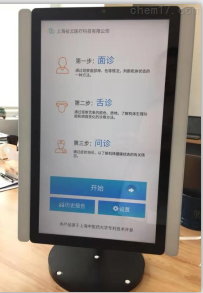
\includegraphics[width=4.5cm]{images/yzy.png}
%     \caption{云中医智能镜}
%     \label{fig:cloudmed}
% \end{figure}

% 云中医智能镜是复旦大学与上海中医药大学联合研发的一款智能产品,外观与一面镜子类似,以镜面作为显示区域与用户交互。用户通过云中医智能镜,可以完成面诊、舌诊、问诊等流程,最终得到健康得分与养生建议。

% 但是云中医智能镜是为诊所与社区环境设计,并没有考虑到用户的日常使用场景,且因为硬件设备体积重量大、造价昂贵,极大地限制了使用场景。
% 同时经过深入调研我们发现云中医智能镜的输入输出模式为端到端模式,把相关的算法都内嵌在一个模型中。
% 对于用户来说整个系统就是一个黑盒,后续研究中本文也发现黑盒模式不利于提高用户对系统的理解和信赖程度。在没有专业人员的指导下,日常场景下使用非常不便。


除面诊仪外,在中医面诊标准化、客观化、信息化的基础上,不少基于中医面诊理论的面诊系统也随之出现。
常见的基于中医的面诊管理系统,其设计的初衷是在诊所的标准环境下服务于医护人员。上海中医药大学的李福凤等基于中医望诊装置\cite{李国正0一种用于中医望诊的三维图像采集装置}的基础上,
利用模式识别相关算法,通过面部分割,面色、光泽、口唇特征分析等方法,实现了一个中医面诊分析与诊断系统\cite{李福凤2016中医面诊分析与诊断系统}。
该系统能够利用采集到的面部数据,对接医院的相关系统,自动为病人建立对应的电子病历,并给出一定的分析结果。
在分析结果的基础上,结合医生的专业诊断得到最终的结果,整体来说简化了面诊的流程,从而达到辅助医生临床诊断的效果。

考虑到诊所环境与日常环境的显著性差异,为诊所环境下设计的面诊系统显然不能直接适用于日常健康场景。
在诊所环境下,医院能够承担昂贵的设备费用,能提供标准的拍摄环境,并且全程有规范的操作流程。
而在日常环境下,用户的文化水平、拍摄环境存在差异,并且需要考虑到长期使用的情况。
复旦大学的林锋等在中医面诊系统调研报告\cite{林锋2019中医面诊系统调研报告}中提到:\myfont{当前面诊仪不够便携,依赖专业医护人员的操作,缺乏友好的人机交互,影响了面诊仪从医疗环境普及到普通家庭环境}。成都中医药大学的宋海贝等在中医面诊健康管理系统的专利\cite{宋海贝2019中医面诊健康管理系统}中也提到:\myfont{目前已经有许多治未病的健康管理系统,并也有对应的面诊智能医疗设备,但现有的面诊智能医疗设备并不适用于日常使用}。
因此宋海贝等以日常健康管理的面诊系统的角度出发,利用智能镜子、智能终端、云端处理器等模块,实现了日常环境下的一个中医面诊健康管理系统。
该系统设计了一个长期监测模块,通过长期的用户数据分析,动态检测用户的健康情况,及时发现用户潜在的健康问题。
相对于为诊所环境设计的面诊系统,该面诊系统考虑到了日常场景中的用户的长期数据,并通过长期数据给出诊断结果。
但除长期数据这一方面外,日常场景下需要考虑的事情可能还有很多,很多细节需要进一步讨论。

\begin{figure}[h]
    \centering
    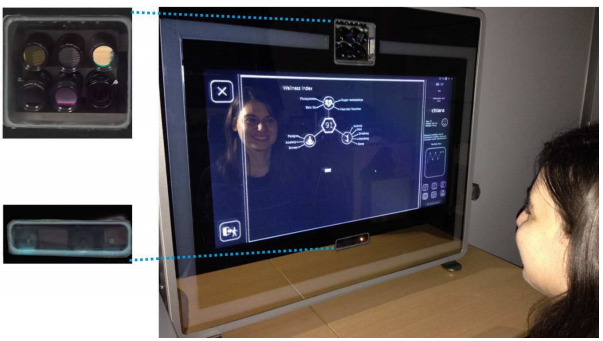
\includegraphics[width=12cm]{images/mirror.png}
    \caption{SEMEOTICONS}
    \label{fig:seme}
\end{figure}
类似的,国外也有类似地考虑到日常环境下面诊系统的系统设计。如图 \ref{fig:seme} 所示,Yasmina Andreu-Cabedo等 \cite{andreu2015mirror}开发了SEMEOTICONS系统。
SEMEOTICONS是一款放在家庭室内环境的镜子,通过摄像头和传感器采集面部信息和体温,监测与心血管疾病相关的疲劳、压力和焦虑等特征,让用户能够监测自己的健康情况,并根据量身定制的健康指南来改善用户的生活方式。
该系统由室内的硬件设备和远程服务器一起完成健康监测的功能,室内设备负责采集数据,远程服务器负责处理数据分析结果。
在生活中照镜子本来就是每个人的日常行为,该研究将读脸技术和健康管理结合起来,并且将应用场景拓展到了日常环境。
他们后续还进行了一次用户体验研究,研究结果表明\cite{coppini2017user} 他们的原型系统的设计被大多数用户所接受: 虽然测试过程非常耗时,大多数参与研究中的志愿者仍然很愿意完成并按计划进行实验,部分志愿者考虑了系统给出的健康指南,甚至因此改变了自己的生活方式。
总的来说,该系统通过将诊断和日常的照镜子的行为结合起来,可以很方便与用户的日常生活融合起来,同时在服务器端也可以方便的实现算法模型的适配和更新。
但是该系统固定在房间的某个位置使用的方式不够便携,同时该系统需要一系列的传感器设备,不仅增加了硬件的成本,部署起来也相对麻烦,而且只能在室内使用。

从上述的研究可以看出,现有的面诊系统大多是为诊所环境设计,部分研究考虑到日常场景的使用问题,但没有系统地用人机交互的研究方法对日常场景下的用户使用进行研究,
将面诊技术应用到日常健康场景还需要进一步深入地探索。

\section{日常健康管理技术}

由上一节我们知道面诊技术的应用和研究有不少,但是它们很少关注日常健康场景。而在人机交互领域,国内外有大量的关于如何设计日常健康场景下健康相关的交互研究。

从研究目的来看,日常健康技术的研究重心偏向于关注患者的日常生活体验,加强患者与医护人员的协作,提高用户的疾病认知等方面\cite{nunes2015self-care}。
从研究的出发点来看,主要可以分为慢性疾病管理和鼓励用户健康生活方式的研究两种\cite{nunes2015self-care},本小节将从这两个方面展开分别介绍。

\subsection{慢性疾病管理}
随着医学、科技和社会的进步,当前的人们享受着比以往时代更加长寿的生活\cite{OlshanskyDEMOGRAPHY}。寿命的增加也间接地造成了慢性病患病率的提高\cite{world2012world}。慢性病作为一种长期的疾病,大多数在目前的医疗条件下是无法治愈的,但是可以通过适当的管理控制病情,因此慢性病管理变得格外重要。

在慢性疾病管理方面,当前研究主要是关于各种类型的慢性疾病的长期管理和追踪技术,用于支持慢性病患者及其护理人员了解病人的身体状态并加强对病情的控制,从而提高用户在患病状态下的生活品质。
如 Lena Mamykina\cite{burgermaster2019personal}团队在安卓平台上研发了一款称为 Platano 的应用,
该系统能够对用户的饮食纪录给出对应的反馈,并通过积分与金钱奖励等机制,逐渐改变用户的饮食习惯。经过实验发现该系统提供的功能能够大大鼓励用户完成血糖管理的任务(如严格控制饮食)。
Kiyoshi Yasuda等\cite{lazar2016evaluation}则研究了如何设计与痴呆病人的远程通讯系统,帮助痴呆病人与家人进行沟通,提高痴呆病人在家保持情绪稳定的时间,改善痴呆病人的日常在家的生活质量。
Amid Ayobi等\cite{ayobi2017quantifying} 通过对多发性硬化病人的日常监测应用的研究,发现日常健康技术可以帮助提高病人的日常控制意识,而不只是监测疾病相关的指标。

在精神健康方面,Jakob E. Bardram等\cite{bardram2013designing}探索了如何设计监测双相情感障碍症的日常应用,研究发现因为移动平台的便携性,患者可以随时携带智能手机,通过系统提醒和实时数据可视化可以提高患者的疾病意识。
同时该系统提供的评估功能相较于纸质表格评估的模式,使用体验大大得到了提高,更加利于用户长期坚持疾病评估。

总的来说,健康管理和患者的日常生活密切相关,慢性病患者需要调整自己的饮食和锻炼等来实现有效的健康管理\cite{nunes2018understanding},因此研究慢性病管理技术对提高慢性病患者的生活水平非常重要。
慢性病管理技术能够帮助用户了解病情的变化,及时对自己的病情变化做出应对行为,更好地评估自己的日常健康行为和更快地适应当前的生活状态\cite{ayobi2017quantifying}。


\subsection{健康行为引导}
在鼓励用户健康生活方面,主要是对各类监测系统的研究。这类系统的功能主要是对用户的各种健康比较相关的指标,能够让用户得到关于自己健康情况的一个反馈,
让处于健康或者亚健康的情况下的用户更加健康地生活。这类监测相关的技术,从对用户监测的指标来看,可以大致分为两类:
\begin{enumerate}

    \item 日常行为的监控:通过监控用户的日常饮食、运动情况等日常行为,培养用户更好的饮食习惯、锻炼习惯等\cite{purpura2011fit4life,Inagawa2013A,bravata2007using,cordeiro2015barriers,lin2006fish, miller2014stepstream}。 例如Yuma Inagawa等人\cite{Inagawa2013A} 开发了一个营养管理和检索系统,根据用户的喜好给出推荐的菜单,用户也可以给出对应的反馈,以此来培养用户健康的健康饮食的观念,进而达到引导用户的行为的效果。

    \item 健康指标的监控:健康指标主要包括生命体征如呼吸、血压、心率,也包括睡眠、体重等\cite{kay2012lullaby,gronvall2013beyond}。
    
\end{enumerate}

例如Stephen Purpura等人\cite{purpura2011fit4life} 利用内有传感器的眼镜、耳机,臂环等可穿戴设备,通过记录用户的饮食、心率、咀嚼动作、体重、血压等健康指标,设计了一个鼓励用户减肥的系统 fit4life; 
Lullaby\cite{kay2012lullaby}是Matthew Kay等人利用光线、声音、温度、运动等传感器研发出来,用于研究干扰用户睡眠因素的系统。
Lullaby系统通过记录和可视化用户的睡眠状态,能够帮助用户识别睡眠中断和环境因素之间的联系。 

% 总结上述的研究我们发现,当前关于日常健康交互技术的研究有很多,涉及各种慢性疾病管理以及各种健康评估和监测的方法,但是目前还缺乏关于日常环境下如何设计基于面部信息进行健康评估的研究。

目前这些日常场景下的健康追踪和监测技术,主要的实现方式还是通过量化采集用户的健康指标相关的数据。那么如何利用其他的健康相关数据,如面部信息,来支持用户的日常健康,在人机交互领域还没有得到深入研究。



\section{本章小结}
本章主要介绍了当前主要的面诊系统设计已经各自的特点和不足,尤其在日常健康场景的系统设计研究目前还十分欠缺。
而人机交互领域在日常健康方面的研究值得我们借鉴。本章后半段介绍了人机交互领域从传统的慢性疾病管理到支持用户更健康生活方式的研究,同时指出当前的日常健康的研究还未探索面部信息作为健康指标的不足不处。